\documentclass[aspectratio=43]{beamer}
\usepackage[latin1]{inputenc}
\usepackage{amsmath}
\usepackage{amsfonts}
\usepackage{amssymb}
\usepackage{makeidx}
\usepackage{graphicx}
\usepackage{array}

% Customization
\mode<presentation>{
\usetheme{CambridgeUS}
\usecolortheme{dolphin}
\setbeamertemplate{navigation symbols}{}
}

%\setbeamertemplate{footline}[frame number]

%TikZ diagrams
\usepackage{tikz}
\usetikzlibrary{patterns}
\usetikzlibrary{arrows,shapes}
\usetikzlibrary{shapes.multipart}
\usetikzlibrary{trees}
\usetikzlibrary{shapes.geometric}
\usetikzlibrary{matrix,arrows}
\usetikzlibrary{positioning}
\usetikzlibrary{calc,through}
\usetikzlibrary{decorations.pathreplacing}
\usepackage{pgffor}

% Define colors
\definecolor{darkgreen}{rgb}{0.0, 0.5, 0.13}
\definecolor{darkblue}{rgb}{0.0, 0.0, 0.55}
\definecolor{darkred}{rgb}{0.55, 0.0, 0.0}

% For using TikZ
\usetikzlibrary{decorations.pathmorphing}
\usetikzlibrary{decorations.markings}
\tikzset{
	vector/.style={decorate, decoration={snake,amplitude=3pt}, draw},
	gluon/.style={decorate, decoration={coil,amplitude=2.5pt},draw},
	provector/.style={decorate, decoration={snake,amplitude=2.5pt}, draw},
	antivector/.style={decorate, decoration={snake,amplitude=-2.5pt}, draw},
	fermion/.style={draw=black, postaction={decorate},
		decoration={markings,mark=at position .55 with {\arrow[draw=black,thick]{>}}}},
	fermionbar/.style={draw=black, postaction={decorate},
		decoration={markings,mark=at position .55 with {\arrow[draw=black,thick]{<}}}},
	fermionnoarrow/.style={draw=black},
	gluon/.style={decorate, draw=black,
		decoration={coil,amplitude=2.5pt, segment length=3pt}},
	gluon2/.style={decorate, draw=black,
		decoration={coil,amplitude=1.75pt, segment length=2.75pt}},
	scalar/.style={dashed,draw=black, postaction={decorate},
		decoration={markings,mark=at position .55 with {\arrow[draw=black]{>}}}},
	scalarbar/.style={dashed,draw=black, postaction={decorate},
		decoration={markings,mark=at position .55 with {\arrow[draw=black]{<}}}},
	scalarnoarrow/.style={dashed,draw=black},
	electron/.style={draw=black, postaction={decorate},
		decoration={markings,mark=at position .55 with {\arrow[draw=black]{>}}}},
	bigvector/.style={decorate, decoration={snake,amplitude=4pt}, draw},
}

% Blocks
\tikzstyle{block} = [draw, rectangle, minimum height = 3em, rounded corners, minimum width = 4em]
\tikzstyle{block2} = [draw, rectangle, minimum height = 3em, rounded corners, minimum width = 7em]
\tikzstyle{circle} = [draw, circle, radius = 1.5]
\tikzstyle{arrow} = [thick,->]
%************************************************************************************************************

% Title and author
\title[Fast predictions for Higgs production]{Fast predictions for Higgs production}
\author{\textbf {Jes\'us Urtasun Elizari}}
%\institute{\textbf {University of Milan}}
\date{Milan, September 2020}

\begin{document}

% Front slide
\begin{frame}

	%\maketitle
	\vspace{1.0 cm}
	
	\center{\color{blue}HTurbo: Fast predictions for Higgs production at the LHC}
	
	\vspace{0.25 cm}
	\center{Jes\'us Urtasun Elizari}
	\center{PhD seminar - Milan, September 2020}

	\begin{figure}
		\minipage{1\textwidth}
		
\includegraphics[width = 3.0 cm]{plots/unimi.png}
		\hfill
		
\includegraphics[width = 3.0 cm]{plots/n3pdf.png}
		\hfill
		
\includegraphics[width = 3.0 cm]{plots/erc.png}
		\endminipage
	\end{figure}

	\vspace{1.0 cm}
	
	{\scriptsize \color{blue} This project has received funding from the European Union$'$s Horizon 2020 research and innovation program under grant agreement No 740006.}

\end{frame}

% Introduction
\begin{frame}

	\frametitle{Outline}
	
	\begin{enumerate}
		\item {\color{blue}QCD in a nutshell}
		\begin{itemize}
			\item The Standard Model $\&$ strong interactions
			\item Running QCD coupling
			\item Factorization theorem
		\end{itemize}
		\item {\color{blue}Dealing with divergences}
		\begin{itemize}
			\item Perturbative QCD and series expansion
			\item Fixed order calculations
			\item Resummation
		\end{itemize}
		\item {\color{blue}HTurbo}
		\begin{itemize}
			\item Higgs production at the LHC: HRes and HqT
			\item HTurbo: Fast predictions for Higgs production
			\item Results $\&$ Conclusions
		\end{itemize}
	\end{enumerate}
	
\end{frame}

% QCD in a nutshell
\begin{frame}

\center{\color{blue}QCD in a nutshell}

\end{frame}

% The Standard model
\begin{frame}

	\frametitle{QCD in a nutshell}
	\framesubtitle{The Standard Model}

	\begin{figure}
		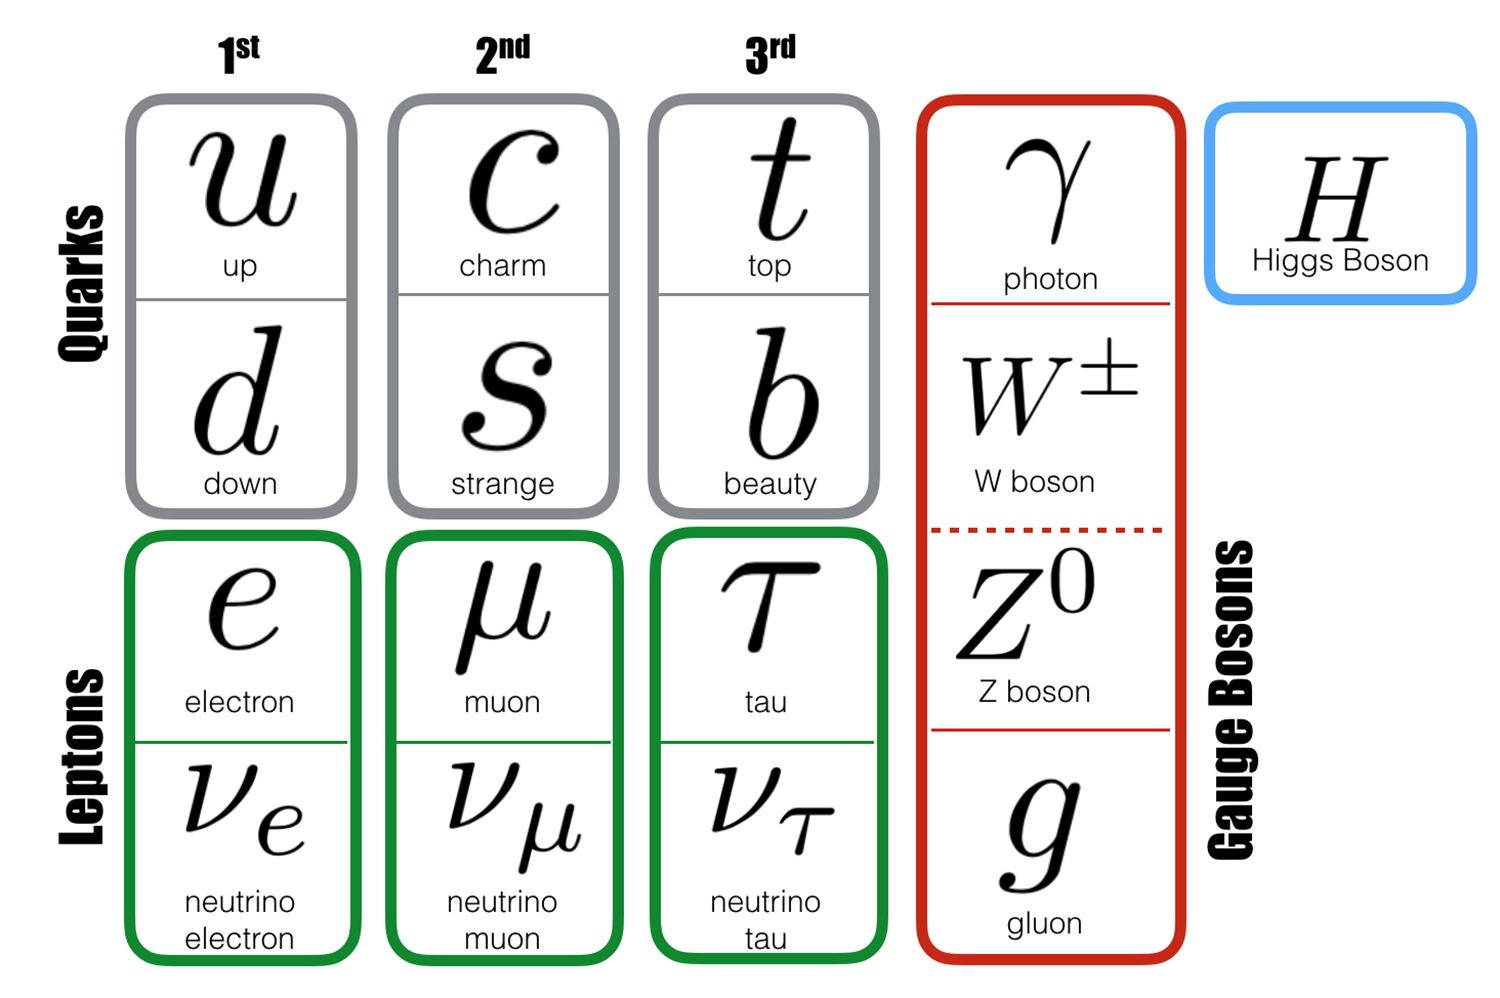
\includegraphics[width = 6 cm]{plots/SM.png}
	\end{figure}
 
	
	Quantum Field Theory describing physics at the TeV scale
	\begin{enumerate}
		\item Fermions composing matter
		\item Bosons mediating interactions
		\item Scalar Higgs generating mass
	\end{enumerate}	
	
\end{frame}

% Explore the proton structure
\begin{frame}

	\frametitle{QCD in a nutshell}
	\framesubtitle{Explore the strong interactions}
	
	How to explore proton's inner structure?
	
	\begin{figure}
		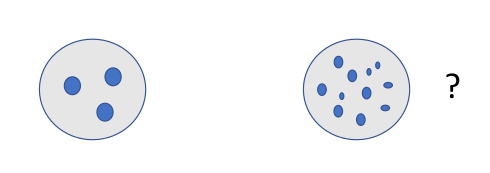
\includegraphics[width = 0.5\linewidth]{plots/protons.png}
	\end{figure}
	
	
	\begin{itemize}
		\item Point-like projectile on the object $\longrightarrow$ DIS
		\item Smash the two objects $\longrightarrow$ LHC physics
	\end{itemize}
	
	{\color{blue}"A way to analyze high energy collisions is to consider any hadron as a composition of point-like constituents $\longrightarrow$ \textbf{partons"} } R.Feynman, 1969 

\end{frame}

% Parton Distribution Functions
\begin{frame}

	\frametitle{QCD in a nutshell}
	\framesubtitle{Parton Distribution Functions}
	
	\begin{figure}
		\minipage{0.5\textwidth}
		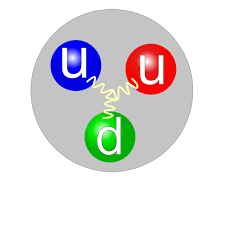
\includegraphics[width = 0.5\linewidth]{plots/proton.png}
		\endminipage\hfill
		\minipage{0.5\textwidth}
		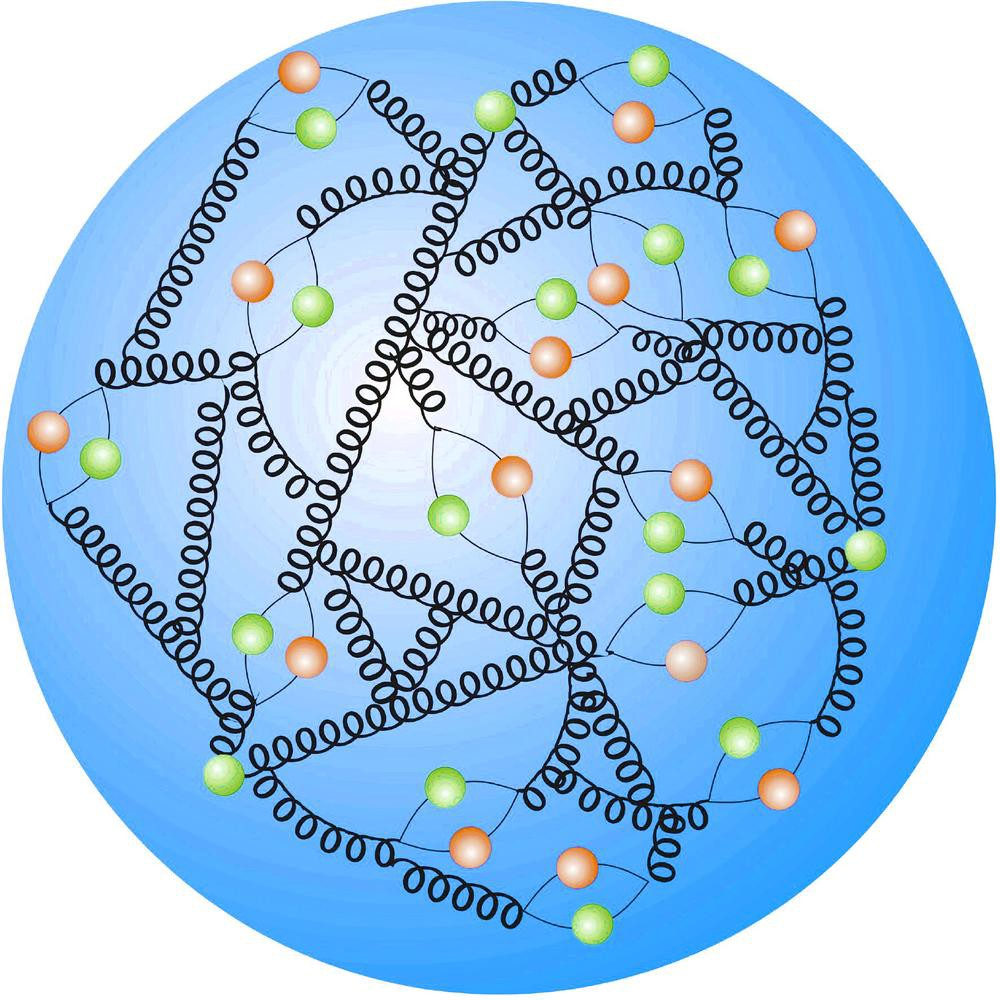
\includegraphics[width = 0.4\linewidth]{plots/proton2.jpg}
		\endminipage
	\end{figure}
	

	\begin{itemize}
		\item Hadrons made of partonic objects $\longrightarrow$ non perturbative physics
		\item Interactions take place only at partonic level $\longrightarrow$ asymptotic freedom
		\item Running coupling given by Renormalization Group Equation (RGE)
	\end{itemize}

	\begin{equation}
		{\color{blue}\mu\frac{d\alpha(\mu)}{d\mu} = \beta(\alpha_{s}(\mu)) = -\sum_{n = 0}^{\infty} \beta_{n} \Big( \frac{\alpha_{s}}{\pi} \Big)^{n + 1}} \nonumber
	\end{equation}

\end{frame}

% Factorization theorem
\begin{frame}

	\frametitle{QCD in a nutshell}
	\framesubtitle{Factorization theorem}
	
	Observables in hadronic events $\longrightarrow$ $\sigma$ is hard to compute
	
	\begin{figure}
		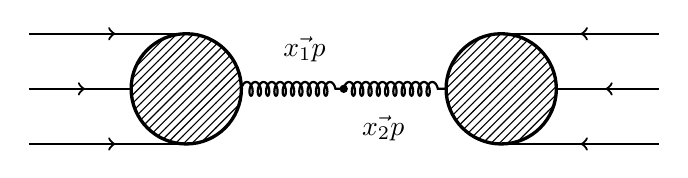
\begin{tikzpicture}
		% Incoming first proton 
		\draw [thick, fermion] (-4, 0.7)--(-2, 0.7);
		\draw [thick, fermion] (-4, 0)--(-2.7, 0);
		\draw [thick, fermion] (-4, -0.7)--(-2, -0.7);
		\draw [thick, very thick, pattern = north east lines] (-2, 0) circle [radius = 0.7];
		% Gluons
		\draw [thick, gluon] (-1.3, 0)--(0, 0);
		\draw [thick, gluon] (0, 0)--(1.3, 0);
		\node at (-0.5, 0.5) {$\vec{x_{1}p}$};
		\node at (0.5, -0.5) {$\vec{x_{2}p}$};
		\draw [thick, very thick, fill = black, pattern = north east lines] (0, 0) circle [radius = 0.03];
		% Incoming second proton
		\draw [thick, very thick, pattern = north east lines] (2, 0) circle [radius = 0.7];
		\draw [thick, fermionbar] (2, 0.7)--(4, 0.7);
		\draw [thick, fermionbar] (2.7, 0)--(4, 0);
		\draw [thick, fermionbar] (2, -0.7)--(4, -0.7);
		\end{tikzpicture}
	\end{figure}
	
	Factorize the problem $\longrightarrow$ Convolute the {\color{red}PDFs}  with the partonic ${\color{blue}\hat{\sigma}_{i j}}$
	
	\begin{equation}
		\sigma = \int_{0}^{1} dx_{1} \; dx_{2} \; {\color{red} f_{\alpha}(x_{1}, \mu_{F}) \ast f_{\beta}(x_{2}, \mu_{F})} \ast {\color{blue}\hat{\sigma}_{\alpha \beta}(\alpha_{s}(\mu_{R}), \mu_{F})} \; \nonumber
	\end{equation}
	
	\begin{itemize}
		\item Partonic {\color{blue}$\hat{\sigma}$} can be computed as perturbative series in $\alpha_{s}$
		\item {\color{red}PDFs} absorb the non perturbative effects, evaluated at $\mu_{F}$
	\end{itemize}

\end{frame}

% Dealing with divergences
\begin{frame}

\center{\color{blue}Dealing with divergences}

\end{frame}

% Partonic cross section and pQCD
\begin{frame}

	\frametitle{Partonic cross section and pQCD}
	\framesubtitle{Why do we need series expansion?}
	\begin{columns}
		
		\column{0.45\textwidth}
		
		\begin{enumerate}
			\item QCD in e+e- collisions
			\item Measure only hadrons in the final state
			\item Factorization theorem helps us to understand short range interactions
		\end{enumerate}
		
		\column{0.45\textwidth}
		\begin{figure}[!htb]
			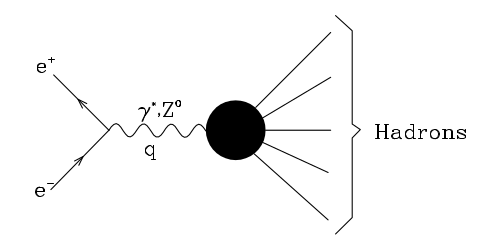
\includegraphics[width = \linewidth]{plots/ee_hadrons.png}
		\end{figure}
	
	\end{columns}

	Write the cross section as a perturbative series
	
\end{frame}

% Perturbative QCD
\begin{frame}

	\frametitle{Perturbative QCD}
	\framesubtitle{Higher order corrections}
	\begin{columns}
	
	\column{0.45\textwidth}
	
	\begin{enumerate}
		\item QCD in e+e- collisions
		\item Measure only hadrons in the final state
		\item Factorization theorem helps us to understand short range interactions
	\end{enumerate}
	
	\column{0.45\textwidth}
	\begin{figure}[!htb]
		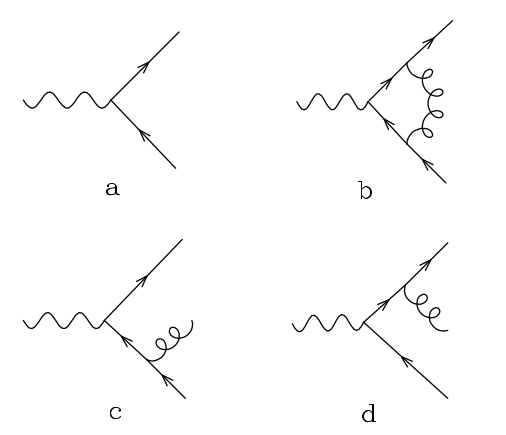
\includegraphics[width = \linewidth]{plots/qcd_corrections.png}
	\end{figure}
	
\end{columns}

\begin{equation}
	\sigma_{q\bar{q}g} = C_{F} \frac{\alpha_{s}}{2\pi} \sigma_{q\bar{q}^{\textrm{Born}}} \int d\cos\theta \frac{dl^{0}}{l} \frac{4}{(1 - cos\theta)(1 + cos\theta)} \nonumber
\end{equation}

	Fixed Order computations diverge!

\end{frame}

% Resummation QCD
\begin{frame}

	\frametitle{Resummation in QCD}
	\framesubtitle{Resumming large logs}

	By truncating the perturbative series at some fixed order, logarithmically enhanced contributions of the form $\ln^{m}(M^{2}/q_{\perp}^{2})$ appear. Then the $q_{\perp}$ distribution need to be evaluated by replacing the partonic cross section as follows
	
	\begin{equation}
		\frac{d\hat{\sigma}_{ab}}{dq_{\perp}^{2}} \rightarrow 
		\Bigg[ \frac{d\hat{\sigma}^{\textrm{res.}}_{ab}}{dq_{\perp}^{2}} \Bigg]_{\textrm{l.a.}} + 
		\Bigg[ \frac{d\hat{\sigma}^{\textrm{fin.}}_{ab}}{dq_{\perp}^{2}} \Bigg]_{\textrm{f.o.}} \nonumber
	\end{equation}

	Resummed expression 
	\begin{equation}
		\frac{d\hat{\sigma}_{ab}^{\textrm{res.}}}{dq_{\perp}^{2}} = \frac{M^{2}}{\hat{s}} \int db \; \frac{b}{2} \; J_{0}(b q_{\perp}) \; \mathcal{W}_{ab}(b, M, \hat{s}; \alpha_{s}(\mu_{R}^{2}), \mu_{R}^{2}, \mu_{F}^{2}) \nonumber
	\end{equation}
	
	Being
	\begin{equation}
		\mathcal{W}_{N}(b, M, \hat{s}; \alpha_{s}(\mu_{R}^{2}), \mu_{R}^{2}, \mu_{F}^{2}) = \mathcal{H} \times exp\{\mathcal{G}\} \nonumber
	\end{equation}

\end{frame}

\begin{frame}

	\frametitle{Resummation in QCD}
	\framesubtitle{Resumming large logs}
		
		\begin{figure}[!htb]
			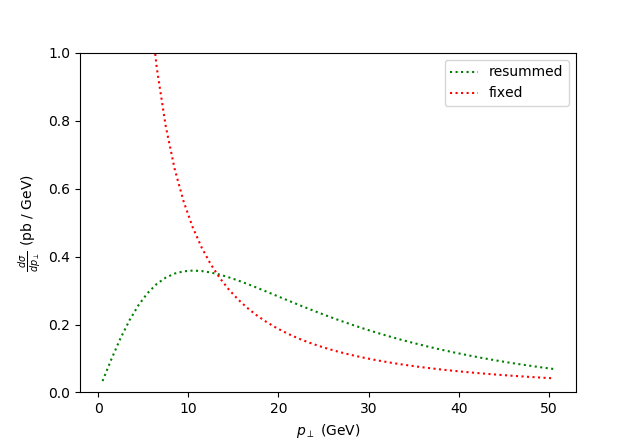
\includegraphics[width = 6 cm]{plots/resummed.png}
		\end{figure}
		
		\begin{enumerate}
			\item FO distribution diverges at small $q_{\perp}$
			\item Sudakov factor kills the divergence
			\item Matched at some intermediate accuracy
		\end{enumerate}

\end{frame}

% HTurbo
\begin{frame}

\center{\color{blue}HTurbo: Fast predictions for Higgs production}

\end{frame}

% HqT and HRes
\begin{frame}

	\frametitle{HqT and HRes}
	\framesubtitle{Predictions for Higgs qT distribution}
	
\end{frame}

% DYturbo
\begin{frame}

	\frametitle{DYTurbo}
	\framesubtitle{Modify a fast version for Drell Yan}

	\begin{enumerate}
		\item Matrix element
		\item Sudakov factor
		\item Hard coefficients
		\item LO integration
	\end{enumerate}

\end{frame}

% Results
\begin{frame}

\frametitle{Results}
\framesubtitle{Comparison HTurbo and HqT}

\begin{figure}
	\minipage{0.32\textwidth}
	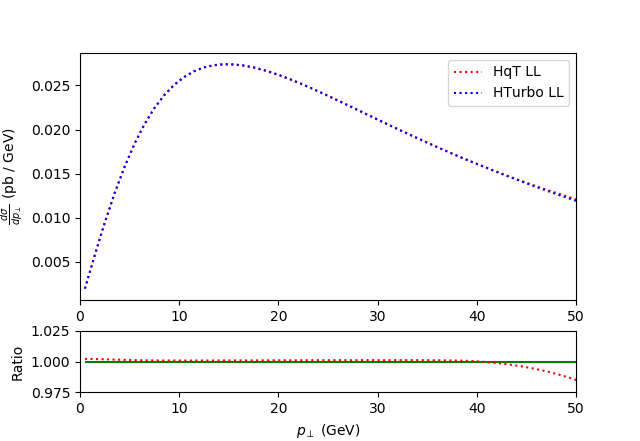
\includegraphics[width = \linewidth]{plots/hturbo_LL.png}
	\endminipage\hfill
	\minipage{0.32\textwidth}
	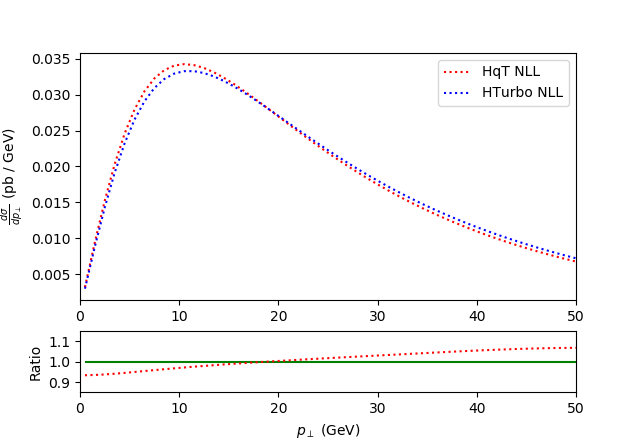
\includegraphics[width = \linewidth]{plots/hturbo_NLL.png}
	\endminipage\hfill
	\minipage{0.32\textwidth}
	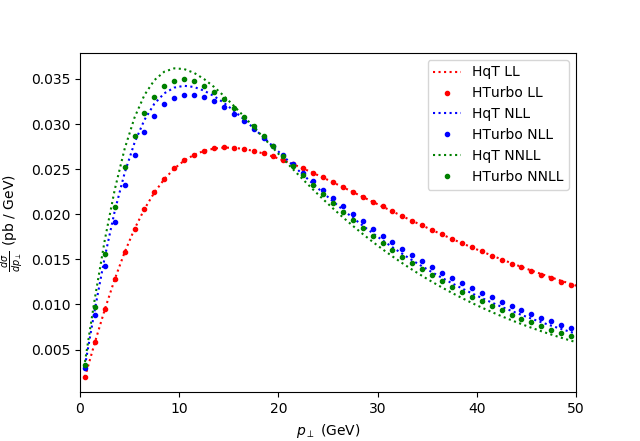
\includegraphics[width = \linewidth]{plots/hturbo_all.png}
	\endminipage
\end{figure}

\begin{itemize}
	\item HTurbo produces qt distributions that match HRes and HqT
	\item Excellent numerical agreement up to NNLO
\end{itemize}

\end{frame}

% Conclusions
\begin{frame}
	
	\frametitle{Summary $\&$ Conclusions}

	\vspace{2.0 cm}
	
	\begin{enumerate}
		\item Fast predictions are required towards the precision era of the LHC
		\item HTurbo produces qt distributions that perfectly match HRes and HqT
		\item Predictions by HTurbo are much faster than any of the existing codes
		\item Next steps: Implement PDF evolution N3LO distributions

	\end{enumerate}

	\vspace{2.0 cm}

	{\small \color{blue} This project has received funding from the European Union$'$s Horizon 2020 research and innovation program under grant agreement No 740006.}

\end{frame}

\end{document}